\documentclass[11pt]{article}
\usepackage{styletemplate}

\setlength{\parindent}{0pt}
\begin{document}

\title{\textbf{Quantum Grothendieck Polynomials for Partial Flags}}
\author{David Yang \and Zoe Markman}
\date{Summer 2024}

\maketitle

\section{Project Goals}

Current Goals include
\begin{itemize}
    \item Extend QKcalc to Quantum Schuberts in partial flags, using universal schubert setup or setup with sigmas
\end{itemize}

Overall project goals and direction include

\begin{itemize}
    \item Candidates for Quantum Grothendiecks for Partial Flags \begin{itemize}
        \item Begin with two-step flags -- good sample cases are $Fl(1, n-1, n)$.
        \item Will likely want to guess and cross-check with Weihong Xu's conjectures.
    \end{itemize}
    \item Multiplication for Quantum Grothendiecks in Full and Partial Flags
\end{itemize}

\section{Background Material}
\subsection{Schubert Polynomials}

Begin with the longest permutation in $S_n$, $w_0 = n \, n-1 \, \dots 1$. The Schubert polynomial for $w_0$ is
\[
    \mathfrak{S}_{w_0}(x) = x_1^{n-1} x_2^{n-2} \dots x_{n-1}.
\]

\begin{definition}[Divided Difference Operator]
The \textit{divided difference operator}, defined on the polynomial ring $\Z[x_1, \dots, x_m]$, is
\[
    \delta_i(f) = \frac{f - s_i(P)}{x_i - x_{i+1}}
\] 
where $s_i(f)$ is the result of interchanging $x_i$ and $x_{i+1}$ in $f$, a polynomial in $\Z[x_1, \dots, x_m]$, for any $i$ between $1$ and $m-1$.
\end{definition}

\begin{definition}[Schubert Polynomials]
The \textbf{Schubert polynomial} corresponding to $w \in S_n$ can be found recursively from $\mathfrak{S}_{w_0}$ by the rule
\[
    \mathfrak{S}_{ws_i} = \delta_i(\mathfrak{S}_w) \text{ if $w(i) > w(i+1)$}.
\]
\end{definition}


When we refer to the complete flag manifold $Fl(1,2,3,4)$, the Schubert polynomials corresponding to the permutations in $S_4$ form the basis for the \textbf{cohomology ring} of the flag manifold.
\begin{definition}[Cohomology Ring]
The \textbf{cohomology ring} of a flag $F$ is written as $H^*(F)$ and it encodes information about the number of intersections of certain Schubert varieties.
\end{definition}
\[
    H^*(Fl(1, 2, 3, 4)) \text{ has basis } \{\mathfrak{S}_w \in S_n \mid w \in S_4 \} 
\]
In general, for a given flag manifold $Fl(d_1, d_2, \dots, d_k)$ with $d_k = n$ we find that the basis for the cohomology corresponds to a subset of the Schubert polynomials of $S_n$:
\[
    H^*(Fl(d_1, d_2, \dots, d_k)) \text{ has basis } \{\mathfrak{S}_w \mid w \in S_n \text{ and has descents } \subseteq \{ d_1, d_2, \dots, n\} \}
\]

Take the specific case of $Gr(2, 4) = Fl(2, 4)$. The basis corresponds to Schubert polynomials of permutations $w \in S_4 \mid w \text{ has descent possibly at $2$}$; the permutations in said basis are Schubert polynomials for $[1\, 2 \mid 3 \,4]$, $[1\,3 \mid 2\,4]$, $[1\, 3 \mid 2\,4]$, $[1\,4 \mid 2\,3]$, $[2\,3 \mid 1\,4]$, $[2\,4 \mid 1\,3]$, and $[3\,4 \mid 1\,2]$. \\

There is an association between the Schubert polynomials corresponding to each of these permutations and an associated Schur polynomial, characterized by the following rule: let $w = w_1 w_2 \dots w_n$. 
\begin{quote}
\textit{If $w_i < w_{i+1}$ for all $i \neq r$ (i.e. there is just one descent at index $r$), $\mathfrak{S}_w$ is the Schur polynomial $s_\lambda(x_1, \dots, x_r)$, where $\lambda = (w_r - r, \dots, w_2 - 2, w_1 - 1)$.}
\end{quote}

The above rule is extremely useful for identifying Schuberts as Schurs. For example, consider the Schubert polynomial corresponding to the permutation $[2\,4 \mid 1\,3]$. There is a descent at index $2$, and so $\lambda = (w_2 - 2, w_1 - 1) = (4 - 2, 2 - 1) = (2, 1)$ and
\[
    \mathfrak{S}_{[2\,4 \mid 1\,3]} = s_{(2, 1)}(x_1, x_2).
\]

The same rule applies for other permutations with one descent. For example, 
\[
    \mathfrak{S}_{[2 \mid 1\,3\,4]} = s_{(1)}(x_1).
\]
In particular, the rule also helps us realize that all Schur polynomials (of a finite number of variables) are Schubert polynomials; any Schur can be reconciled with a given permutation with one descent, which corresponds to a Schubert polynomial. \\

\textit{Additional Info: Schubert polynomials can be realized through pipe dreams or rc-graphs -- see \href{https://sites.math.washington.edu/~billey/papers/bjs.pdf}{Billey-Jockusch-Stanley} for more information.}

\subsection{Cohomology and Quantum Cohomology}
\subsubsection{Introduction and Algebraic Representations}
In the previous section, we introduced cohomology rings. There are also quantum cohomology and quantum k-theoretic rings. We introduce the former below.
\begin{definition}[Quantum Cohomology Ring]
The \textbf{quantum cohomology ring} of a flag $F$ is denoted $QH^*(F)$ and it encodes information about the number of algebraic curves passing through multiple Schubert varieties (more specifically, 3-point, genus-zero Gromov-Witten invariants).
\end{definition}
Algebraically, the cohomology and quantum cohomology rings can be represented as follows
\[
    H^*(Fl_n) \cong \faktor{\Z[x_1, \dots, x_n]}{\{ e_i(n) \mid i \in \{1, \dots, n \}\}}
\]
and 
\[
    QH^*(Fl_n) \cong \faktor{\Z[x_1, \dots, x_n][q_1, \dots, q_{n-1}]}{\{ E_i(n) \mid i \in \{1, \dots, n \}\}}
\]
where each $E_i(n)$ corresponds to the quantized standard elementary monomial (see section below).

\subsubsection{Bases for Cohomology Ring}
As we have just seen, one basis for the cohomology ring $H^*(Fl_n)$ is the set of Schubert polynomials corresponding to each permutation in $S_n$, or
\[
    \{ \mathfrak{S}_w(x_1, \dots, x_n) \mid w \in S_n \}.
\]

The set of Schubert polynomials is a positive basis; indeed, the Littlewood-Richardson Rule for Schur polynomials generalizes to Schuberts, and we have
\[
    \mathfrak{S}_u \mathfrak{S}_v = \sum_{w} c_{uv}^w \mathfrak{S}_w
\]
where each $c_{uv}^w$ is a unique (because the Schuberts are a basis) nonnegative coefficient. \\

Another well-known basis is known as the \textbf{\textit{standard elementary monomials}}, of the form
\[
    \{e_{i_1}(1) \cdots e_{i_{n-1}}(n-1) \mid 0 \leq i_k \leq k \}
\]
where each $e_k(p)$ corresponds to the elementary symmetric polynomial of degree $k$ in $p$ variables $x_1, \dots, x_p$. Contrary to the previous Schubert basis, this is not a positive basis. For example, consider $Fl(3)$ and the product $e_1(1) \cdot e_1(1).$ We have that
\begin{align*}
    e_1(1) \cdot e_1(1) &= x_1^2 \\
    &= x_1(x_1 + x_2) - x_1x_2 \\
    &= e_1(1)e_1(2) - e_2(2).
\end{align*}

Note that each of these bases has precisely $n!$ entries, a defining characteristic for the bases of a complete flag manifold. \\

\subsubsection{Quantized Standard Elementary Monomials: Dynkin and Matrix Approaches}
The quantized standard elementary monomials in both full and partial flag manifolds can be realized from two different methods. We begin with a discussion of the quantized standard elementary monomials in the full flag case. From Fomin-Gelfand-Postnikov (FGP), we can realize the quantized standard elementary monomial through the characteristic polynomial of the matrix
\[
    G_n = \begin{bmatrix}
    x_1 & q_1 & 0 & \dots & 0 \\
    -1 & x_2 & q_2 & \dots & 0 \\
    \vdots & \vdots & \vdots & \ddots & \cdots \\
    0 & 0 & 0 & \dots & x_n
    \end{bmatrix},
\]
which is constructed with the $x_i$ terms on the main diagonal, the quantum $q$ terms on the superdiagonal, $-1$ terms on the subdiagonal, and $0$'s elsewhere. \\

With the property
\[
    \det(1 + \lambda G_n) = \sum\limits_{i=0}^n E_i(n) \lambda^i,
\]
we realize the quantized standard elementary monomial $E_{i-j}(n)$ as the coefficient of the $\lambda^j$ term in $\det(1 + \lambda G_n)$. \\

\begin{eg}[Matrix Approach for Quantized Monomials in $Fl_3$]

We will begin by using the matrix approach. Note that
\[
    G_3 = \begin{bmatrix}
    x_1 & q_1 & 0 \\
    -1 & x_2 & q_2 \\
    0 & -1 & x_3
    \end{bmatrix}.
\]
We see that $1 + \lambda G_3 = \begin{bmatrix}
    1 + \lambda x_1 & \lambda q_1 & 0 \\
    -\lambda & 1 + \lambda x_2 & \lambda q_2 \\
    0 & -\lambda & 1 + \lambda x_3
    \end{bmatrix}$
so $\det (1 + \lambda G_1)$ is the determinant of the upper left $1 \times 1$ corner of $G_3$, $\det (1 + \lambda G_2)$  is the determinant of the upper left $2 \times 2$ corner of $G_3$, and $\det (1 + \lambda G_3)$ is the determinant of the whole matrix. We get

\[
    \det (1 + \lambda G_1) = 1 + \lambda x_1,
\]
\begin{align*}
    \det (1 + \lambda G_2) &= (1+\lambda x_1)(1+\lambda x_2) + \lambda^2 q_1 \\
    &= 1 + \lambda (x_1 + x_2) + \lambda^2 (x_1x_2 + q_1).
\end{align*}

Recognizing the quantum standard elementary monomials as the coefficients of the respective determinants, we get that
\[
    \boxed{E_1(1) = x_1, E_1(2) = x_1 + x_2, \text{ and } E_2(2) = x_1x_2 + q_1}.
\]
\end{eg}

\vspace{0.5cm}
Alternatively, one can recognize the standard elementary monomials through the use of Dynkin diagrams. Consider some flag manifold $Fl(d_1, \dots, d_n)$; by convention, $d_0 = 0$. The number of quantum terms $q_i$ corresponds to the number of steps in the flag, which is $n-1$. Each quantum term $(-1)^{d_{i+1} - d_{i} + 1}q_i$ covers $x_{d_{i-1} + 1}$ to $x_{d_{i+1}}$, for $i$ from $1$ to $n-1$, per equation (18) in Fulton's Universal Schubert article. \\

The \textit{\textbf{Dynkin diagram}} represents the relationships between the $x$ and $q$ terms, and can be used to determine the quantized standard elementary monomials. \\

In general, recall that the standard elementary monomial $e_i(j)$ represents the sum of monomials of degree $i$ from the set $\{x_1, \dots, x_j\}$ that cover each $x_i$ at most once. \\

Similarly, the \textit{quantized standard elementary monomial} $E_i(j)$ represents the sum of monomials of degree $i$ from the set $\{x_1, \dots, x_j\}$ and corresponding $q$ entries that cover each $x_i$ at most once. \\

\begin{eg}[Dynkin Approach for Quantized Monomials in $Fl_3$]
The Dynkin Diagram for $Fl_3$ is as follows:
\begin{center}
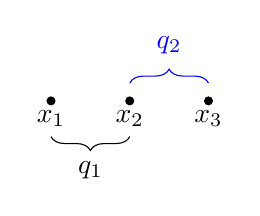
\begin{tikzpicture}
\filldraw[black] (0, 0) circle (0.05);
\filldraw[black] (1, 0) circle (0.05);
\filldraw[black] (2, 0) circle (0.05);
\draw [decorate,decoration={brace,amplitude=5pt,mirror,raise=3ex}]
  (0,0) -- (1,0) node[midway,yshift=-2.5em]{$q_1$};
  \draw [decorate,decoration={brace,amplitude=5pt,raise=1.5ex},color={blue}]
  (1,0) -- (2,0) node[midway,yshift=2em]{$q_2$};
\node[below] at (0, 0) {$x_1$};
\node[below] at (1, 0) {$x_2$};
\node[below] at (2, 0) {$x_3$};
\end{tikzpicture}
\end{center}
We can easily identify the corresponding quantized standard elementary monomials:
\[
    \boxed{E_1(1) = x_1, E_1(2) = x_1 + x_2, E_2(2) = x_1x_2 + q_1},
\]
which match the matrix approach calculations.
\end{eg}


\begin{remark}
The above two approaches are equivalent formulations for determining the quantized standard elementary monomials. The diagram approach can be generalized to partial flag manifolds as is (see below), whereas the matrix approach has a similar but slightly more complicated structure in the partial flag case.
\end{remark}

\begin{eg}[Dynkin Example in $Fl(1, 2, 4)$]
Consider the following Dynkin diagram corresponding to the flag manifold $Fl(1, 2, 4)$. by the above formulalation, $(-1)^{2-1+1}q_1 = q_1$ spans $x_{d_0 + 1} = x_1$ to $x_{d_1} = x_3$ and $(-1)^{4-2+1}q_2 = -q_2$ spans $x_{d_1 + 1} = x_2$ to $x_{d_2} = x_4$. 
\begin{center}
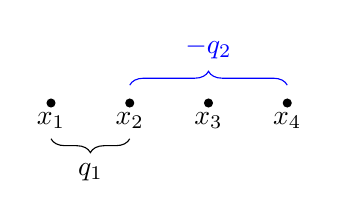
\begin{tikzpicture}
\filldraw[black] (0, 0) circle (0.05);
\filldraw[black] (1, 0) circle (0.05);
\filldraw[black] (2, 0) circle (0.05);
\filldraw[black] (3, 0) circle (0.05);
\draw [decorate,decoration={brace,amplitude=5pt,mirror,raise=3ex}]
  (0,0) -- (1,0) node[midway,yshift=-2.5em]{$q_1$};
  \draw [decorate,decoration={brace,amplitude=5pt,raise=1.5ex},color={blue}]
  (1,0) -- (3,0) node[midway,yshift=2em]{$-q_2$};
\node[below] at (0, 0) {$x_1$};
\node[below] at (1, 0) {$x_2$};
\node[below] at (2, 0) {$x_3$};
\node[below] at (3, 0) {$x_4$};  
\end{tikzpicture}
\end{center}

We have that
\[
    E_4(4) = x_1x_2x_3x_4 + q_1x_3x_4 - x_1q_2.
\]
\textit{Note: this notation is slightly different from the quantum Giambelli notation in Ciocan-Fontanine. Here, $E_i(j)$ refers to the quantized standard elementary monomial of degree $i$ covering variables $x_1, \dots, x_j$.}
\end{eg}

\vspace{0.25cm}

The matrix approach can also be adapted to calculate the Quantized Standard Elementary Monomials in Partial Flags, following a procedure discussed in Ciocan-Fontanine. \\

Consider $F = Fl(n_1, \dots, n_k)$. The matrix setup is as follows: we define $\sigma_1^1, \dots, \sigma_{n_1}^1, \sigma_1^2, \dots, \sigma_{n_2 - n_1}^2$, $\dots, \sigma_1^{k+1}, \dots, \sigma_{n-n_k}^{k+1}$ to be $n$ independent variables, and define $A_n$ to be a block diagonal matrix $\mathrm{diag}(D_1, \dots, D_{k+1})$ where
\[
    D_j \coloneqq \begin{bmatrix}
        \sigma_1^j & \sigma_2^j & \dots & \sigma_{n_j - n_{j-1} - 1}^j & \sigma_{n_j - n_{j-1}}^j \\
        -1 & 0 & \dots & 0 & 0 \\
        \vdots & \vdots & \dots & \vdots & \vdots \\
        0 & 0 & \dots & -1 & 0.
    \end{bmatrix}
\]

A result by Borel (0.1 in Ciocan-Fontanine) tells us that there is an isomorphism 
\[
    \boxed{H^*(F) \cong \faktor{\Z[\sigma_1^1, \dots, \sigma_{n_1}^1, \dots, \sigma_1^{k+1}, \dots, \sigma_{n-n_k}^{k+1}]}{(g_1, \dots, g_n)}}
\]
where $g_1, \dots, g_n$ are the coefficients of the characteristic polynomial of the matrix $A_n$. \\

In particular, if we interpret a given partial flag manifold, if we interpret each $\sigma_i^j$ as the $i$th elementary symmetric polynomial in variables $x_{n_{j-1} + 1}, \dots, x_{n_j}$, we can recover the Schubert polynomials, and the Schubert polynomials serve as the Giambelli polynomials which are associated with Schubert classes in our partial flag manifold. \\

Just as importantly, we can obtain a  presentation of the quantum cohomology ring of any partial flag manifold $F$, matching (0.3) in Ciocan-Fontanine. If we define $B_n = (b_{lm})_{1 \leq l, m \leq n}$ to be the matrix with entries
\[
b_{lm} = \begin{cases}
    (-1)^{n_{j+1} - n_j + 1} q_j & \text{ if $l = n_{j-1} + 1$ and $m = n_{j+1}$, for $1 \leq j \leq k$} \\
    -1 & \text{ if $l = n_{j} + 1$ and $m = n_{j}$ for $1 \leq j \leq k$} \\
    0 & \text{ otherwise},
\end{cases}
\]

then there is an isomorphism
\[
    \boxed{QH^*(F) \cong \faktor{\Z[\sigma_1^1, \dots, \sigma_{n_1}^1, \dots, \sigma_1^{k+1}, \dots, \sigma_{n-n_k}^{k+1}][q_1, \dots, q_k]}{(G_1, \dots, G_n)}}
\]
where the $G_1, \dots, G_n$ are the coefficients of the characteristic polynomial of $A_n^q = A_n + B_n$. \\

We can use this matrix setup and mirror the procedure for the full flag case to determine the quantized standard elementary monomials in partial flags. 

\begin{theorem}[Ciocan-Fontanine page 499(iii)]
Consider the flag $F = Fl(n_1, n_2, \dots, n_k)$. The quantum Giambelli polynomial $G_i^j$ (corresponding to the standard elementary monomial $E_i(n_j)$ discussed above) satisfies
\[
    G_{i}^j \text{ is the coefficient of } \lambda^{i-j} \text{ in } \det (A_{n_j}^q + \lambda I)
\] 
where $A_{n_j}^q$ is the upper left $n_j \times n_j$ submatrix of the $A_n^q$ matrix defined above.
\end{theorem}

\begin{eg}[$Fl(1, 2, 4)$ Calculations \textcolor{red}{Fix example}]
\begin{align*}
A_4^q = A_4 + B_4 &=
\begin{bmatrix}
x_1 & 0 & 0 & 0 \\
0 & x_2 & 0 & 0 \\
0 & 0 & \sigma_1^3 & \sigma_2^3 \\
0 & 0 & -1 & 0
\end{bmatrix} + 
\begin{bmatrix}
0 & q_1 & 0 & 0 \\
-1 & 0 & 0 & -q_2 \\
0 & -1 & 0 & 0 \\
0 & 0 & 0 & 0
\end{bmatrix}
=
\begin{bmatrix}
    x_1 & q_1 & 0 & 0 \\
    -1 & x_2 & 0 & -q_2 \\
    0 & -1 & \sigma_1^3 & \sigma_2^3 \\
    0 & 0 & -1 & 0
\end{bmatrix} \\
&= 
\begin{bmatrix}
    x_1 & q_1 & 0 & 0 \\
    -1 & x_2 & 0 & -q_2 \\
    0 & -1 & x_3 + x_4 & x_3x_4 \\
    0 & 0 & -1 & 0
\end{bmatrix}.
\end{align*}

Note that 
\[
    \det(A_2^q + \lambda I) = \left|
    \begin{bmatrix}
    x_1 + \lambda & q_1 \\
    -1 & x_2 + \lambda
    \end{bmatrix}
    \right| = (x_1x_2 + q_1) + \lambda(x_1 + x_2) + \lambda^2
\]
so $E_2(2) = x_1x_2 + q_1$ and $E_1(2) = x_1 + x_2$. \\

Similarly, 
\[
    \det(A_3^q + \lambda I) = \left|
    \begin{bmatrix}
    x_1 + \lambda & q_1 & 0 \\
    -1 & x_2 + \lambda & 0 \\
    0 & -1 & x_3 + x_4 + \lambda
    \end{bmatrix}
    \right| = (x_1x_2x_3 + x_1x_2x_4) + \lambda
\]

\end{eg}
\subsection{Quantum Schubert Polynomials}
\subsubsection{Complete Flag Case}
\textbf{\textit{Quantum Schubert polynomials}} arise as ``quantized'' versions of the Schubert polynomials. Consider the Schubert polynomial $\mathfrak{S}_{[3 \, 1 \, 2]}$ in $S_3$. One can find, using the divided difference operator, that $\mathfrak{S}_{[3 \, 1 \, 2]} = x_1^2$ -- from the above example, we know that this can also be rewritten in the standard elementary monomial basis:
\begin{align*}
    \mathfrak{S}_{[3 \, 1 \, 2]} &= x_1^2 \\
    &= e_1(1) e_1(2) - e_2(2).
\end{align*}

To determine the corresponding quantum Schubert polynomial, we simply replace each of the standard elementary monomials with their quantized versions (represented by capital letters), so

\begin{align*}
    \mathfrak{S}_{[3 \, 1 \, 2]}^q &= E_1(1) E_1(2) - E_2(2) \\
    &= x_1(x_1 + x_2) - (x_1x_2 + q_1) \\
    &= x_1^2 - q_1
\end{align*}

The quantum Schubert polynomials serve as a basis for the quantum cohomology of $Fl(3)$. As we saw in the cohomology case, in general, the basis for the quantum cohomology of a partial flag $Fl(d_1, d_2, \dots, d_k)$ $ \leftrightarrow \{\mathfrak{S}_w \in S_n \mid w \text{ has descents } \subseteq \{ d_1, d_2, \dots, d_k\} \}$. \\

The following is a Quantum Monk rule for products of Quantum Schuberts in Complete Flags:
\begin{theorem*}[Quantum Monk for Quantum Schubert in Complete Flags, FGP (584)]
Let $t_{ab}$ be the transposition of positions $a$ and $b$.
    \[
        \mathfrak{S}_{s_r}^q \mathfrak{S}_{w}^q = \sum \mathfrak{S}_{wt_{ab}}^q + \sum q_{cd}\mathfrak{S}_{wt_{cd}}^q
    \]
    where the first sum is over $a \leq r < b$ such that $l(wt_{ab}) = l(w) + 1$ and the second sum is over $c \leq r < d$ such that $l(wt_{cd}) = l(w) - l(t_{cd}) = l(w) - 2(d - c) + 1$. \textit{note: $q_{cd} = q_c q_{c+1} \dots q_{d-1}$.}
\end{theorem*}

\subsubsection{Partial Flag Case}
\textcolor{red}{Universal Schubert by Fulton}

\subsection{Grothendieck Polynomials}

Begin with the longest permutation in $S_n$, $w_0 = n \, n-1 \, \dots 1$. The Grothendieck polynomial of $w_0$ is the same as the Schubert polynomial for $w_0$:
\[
    \mathfrak{G}_{w_0}(x) = x_1^{n-1} x_2^{n-2} \dots x_{n-1}.
\]
\begin{definition}[Grothendieck Polynomials]
Let $\delta_i = \frac{f - s_i(f)}{x_i - x_{i+1}}$ be the divided difference operator, and let $\pi_i = \delta_i(1-x_{i+1})$. 

The Grothendieck polynomials for $w \in S_n$ are defined as
\begin{align*}
    \mathfrak{G}_w(x_1, x_2, \ldots, x_n) &= \pi_{w^{-1}w_0}(x_1^{n-1} x_2^{n-2} \ldots x_{n-1}) 
\end{align*}
\end{definition}


\begin{definition}[Equivalent Formulations of Grothendiecks]
The \textit{isobaric divided difference operator} is defined as
\[
    \overline{\delta}_i(f) = \delta_i[(1-x_{i+1})f]
\] 
and the \textbf{Grothendieck polynomial} corresponding to $w \in S_n$ can be found recursively from $\mathfrak{G}_{w_0}$ by the rule
\[
    \mathfrak{G}_{ws_i} = \overline{\delta}_i(\mathfrak{G}_w) \text{ if $w(i) > w(i+1)$}
\]
\end{definition}

Some code on computing Grothendieck polynomials in Sage: \href{https://wiki.sagemath.org/combinat/MultivariatePolynomials}{how to compute these in sage}!

Note that the lowest degree homogenous part of $\mathfrak{G}_w$ is given by $\mathfrak{S}_w$ (the corresponding Schubert polynomial). 

\begin{theorem}[Grothendieck Pieri, from Lenart and Maeno]
    \begin{equation*}
        \mathfrak{G}_wg_p^k = \sum_\gamma m_p(\gamma) \mathfrak{G}_{\text{end}(\gamma)}
    \end{equation*} 
    where the sum is over all $k$-Pieri chain $\gamma$ on the infinite symmetric group that begin at $w$.

    We define $g_p^k = \mathfrak{G}_{c[k,p]} = \sum_{i=p}^k (-1)^{i-p} {{i-1}\choose{p-1}} e_i^k$. We let $\gamma$ denote a $k$-Pieri chain (see definition 2.14), $m_p(\gamma) = (-1)^{l(\gamma) -p}$ times the number of $p$-markings of $\gamma$.
\end{theorem}
The $k$-Pieri chain looks complicated — The monk formula covers the case when $p = 1$, and seems much nicer. I think the $k$-Pieri chain is the big (gross) thing that lets you generalize.

\begin{definition}[Quantum Grothendieck Polynomials]
    The \textbf{Quantum Grothendieck polynomial} $\mathfrak{G}_w^q$, for $w \in S_n$, is
    \begin{equation*}
        \mathfrak{G}_w^q = \hat{Q}(\mathfrak{G}_w) \in \Z[q,x]
    \end{equation*}
\end{definition}
The quantum Grothendiecks for $S_3$ are in example 3.19 of Lenart-Maeno, and a combinatorial formula is given later in the paper. \\

\begin{theorem}[Quantum Monk for Grothendieck -- Theorem 6.4 in LeM]

We have
\begin{equation*}
    \G_w^q \G_{s_k}^q = \sum_\pi (-1)^{l(\pi)- 1}q(\pi) \G_{end(\pi)} ; 
\end{equation*}
the summation is over all nonempty paths $\pi$ in the quantum $k$-Bruhat graph (of $S^\infty$) of the form 
\begin{equation*}
    w = w_0 \rightarrow w_1 \rightarrow \ldots \rightarrow w_s = \text{end}(\pi)
\end{equation*}
where $(a_1, b_1) \prec (a_2,b_2) \prec \ldots \prec (a_s,b_s)$.
\end{theorem}

For calculations with quantum Grothendiecks, there is the following \href{https://ow3.math.rutgers.edu/~asbuch/equivcalc/}{Maple Package for Quantum Grothendiecks}.

\section{Quantum Grothendiecks in Partial Flags}


\newpage

\section{Appendix}

\begin{table}[!h]
\centering
\caption{Schuberts for $Fl(1, 3, 4)$}
\begin{tabular}{|c|c|p{10cm}|}
\hline
\textbf{Permutation} & \textbf{Quantum Schubert} \\ \hline
1234 & 1 \\ \hline 
1243 & $x_1 + x_2 + x_3$ \\ \hline
1342 & $x_1(x_2 + x_3) + x_2x_3$ \\ \hline
2134 & $x_1$ \\ \hline
2143 & $x_1(x_1 + x_2 + x_3)$ \\ \hline
2341 & $x_1x_2x_3 - q_1$ \\ \hline 
3124 & $x_1^2$ \\ \hline
3142 & $x_1^2(x_2 + x_3) + q_1$ \\ \hline
3241 & $x_1(x_1x_2x_3 - q_1)$ \\ \hline
4123 & $x_1^3 - q_1$ \\ \hline
4132 & $x_1(x_1^2(x_2 + x_3) + q_1)$ \\ \hline
4231 & $x_1^2(x_1x_2x_3 - q_1)$ \\ \hline
\end{tabular}
\end{table}

\begin{table}[!h]
\centering
\caption{Schuberts for $Fl(1, 2, 4)$}
\begin{tabular}{|c|c|p{10cm}|}
\hline
\textbf{Permutation} &  \textbf{Quantum Schubert} \\ \hline
1234 & 1 \\ \hline 
1324 & $x_1 + x_2$ \\ \hline
1423 & $x_1^2 + x_1x_2 + x_2^2 - q_1$ \\ \hline
2134 & $x_1$ \\ \hline
2314 & $x_1x_2 + q_1$ \\ \hline
2413 & $(x_1+x_2)(x_1x_2 + q_1)$ \\ \hline 
3124 & $x_1^2 - q_1$ \\ \hline
3214 & $x_1(x_1x_2 + q_1)$ \\ \hline
3412 & $(x_1x_2 + q_1)^2$ \\ \hline
4123 & $x_1^3 + q_1(-2x_1 - x_2)$ \\ \hline
4213 & $-(-x_1^2 + q_1)(x_1x_2 + q_1)$ \\ \hline
4312 & $x_1(x_1x_2 + q_1)^2$ \\ \hline
\end{tabular}
\end{table}


\begin{table}[!h]
\centering
\caption{Grothendiecks for $Fl(3)$}
\begin{tabular}{|p{2cm}|c|p{10cm}|}
\hline
Permutation &  Grothendieck  &  Quantum Grothendieck  \\ \hline
123 & 1 & 1 \\ \hline
132 & $-x_1x_2 + x_1 + x_2$ & $x_1x_2q_2 - x_1x_2 - x_1q_2 - x_2q_2 + x_1 + x_2 + q_2$ \\ \hline
213 & $x_1$ & $-x_1q_1 + x_1 + q_1$ \\ \hline
231 & $x_1x_2$ & $-x_1x_2q_2 + x_1x_2 - x_1q_1 + x_1q_2 + q_1$ \\ \hline
312 & $x_1^2$ & $
    x_1^2q_1^2 + x_1x_2q_1q_2  - 2x_1^2q_1 - x_1x_2q_1 - 2x_1q_1^2 - x_1q_1q_2 
    - x_2q_1q_2 + x_1^2 + 3x_1q_1 + x_2q_1 + q_1^2 + q_1q_2 - q_1$ \\ \hline 
321 & $x_1^2x_2$ & $x_1^2x_2q_1q_2 - x_1^2x_2q_1 + x_1^2q_1^2 - x_1^2x_2q_2 - x_1^2q_1q_2 - x_1x_2q_1q_2 + x_1^2x_2 - x_1^2q_1 + x_1x_2q_1 - 2x_1q_1^2 + x_1^2q_2 + x_1q_1q_2 + x_1q_1 + q_1^2$ \\ \hline 
\end{tabular}
\end{table}


\newpage

Multiplication Tables for $Fl(3)$
\begin{table}[!h]
\centering
\caption{Quantum Schuberts for $Fl(3)$}
\begin{tabular}{|p{1.2cm}|p{2cm}|p{3cm}|p{2cm}|p{2cm}|p{2cm}|p{2cm}|}
\hline
$\times$ & \textbf{X[123]} & \textbf{X[132]} & \textbf{X[213]} & \textbf{X[231]} & \textbf{X[312]} & \textbf{X[321]} \\ \hline
\textbf{X[123]} & X[1] & X[132] & X[213] & X[231] & X[312] & X[321] \\ \hline 
\textbf{X[132]} & X[132] & $q_2X[1]+X[231]$ & $X[231]+X[312]$ & $q_2X[213]$ & $X[321]$ & $q_1q_2X[1]+q_2X[312]$  \\ \hline
\textbf{X[213]} & X[213] & X[231]+X[312] & $q_2X[312]$ & X[321] & $q_1X[132]$ & $q_1q_2X[1]+q_1X[231]$ \\ \hline 
\textbf{X[231]} & X[231] & $q_2X[213]$ & X[321] & $q_2X[312]$ & $q_1q_2X[1]$ & $q_1q_2X[132]$\\ \hline
\textbf{X[312]} & X[312] & X[321] & $q_1X[132]$ & $q_1q_2X[1]$ & $q_1X[231]$ & $q_1q_2X[213]$ \\ \hline
\textbf{X[321]} & X[321] & $q_1q_2X[1]+q_2X[312]$ & $q_1q_2X[1]+q_1X[231]$ & $q_1q_2X[132]$ & $q_1q_2X[213]$ & $q_1q_2X[3,1,2]$ \\ \hline
\end{tabular}
\end{table}


\begin{table}[!h]
\centering
\caption{Quantum Grothendiecks for $Fl(3)$}
\begin{tabular}{|p{1.2cm}|p{1.2cm}|p{2.5cm}|p{2.5cm}|p{2cm}|p{2cm}|p{2.6cm}|}
\hline
$\times$ & \textbf{X[123]} & \textbf{X[132]} & \textbf{X[213]} & \textbf{X[231]} & \textbf{X[312]} & \textbf{X[321]} \\ \hline
\textbf{X[123]} & X[1] & X[132] & X[213] & X[231] & X[312] & X[321] \\ \hline 
\textbf{X[132]} & $X[132]$ & $q_2X[1, 2, 3] - q_2X[2, 1, 3] + X[2, 3, 1]$ & $X[2, 3, 1] + X[3, 1, 2] - X[3, 2, 1]$ & $q_2X[2, 1, 3]$ & $X[3, 2, 1]$ & $q_1q_2X[1, 2, 3] - q_1q_2X[1, 3, 2] + q_2X[3, 1, 2]$  \\ \hline
\textbf{X[213]} & X[213] & $X[2, 3, 1] + X[3, 1, 2] - X[3, 2, 1]$ & $q_1X[1, 2, 3] - q_1X[1, 3, 2] + X[3, 1, 2]$
& $q_1X[1, 2, 3] - q_1X[1, 3, 2] + X[3, 1, 2]$ & $q_1X[1, 3, 2]$ & $q_1q_2X[1, 2, 3] - q_1q_2X[2, 1, 3] + q_1X[2, 3, 1]$ \\ \hline 
\textbf{X[231]} & $X[231]$ & $q_2X[2, 1, 3]$ & $X[3, 2, 1]$ & $q_2X[3, 1, 2]$& $q_1q_2X[1, 2, 3]$& $q_1q_2X[1, 3, 2]$ \\ \hline
\textbf{X[312]} & $X[312]$ & $X[3, 2, 1]$ & $q_1X[1, 3, 2]$& $q_1q_2X[1, 2, 3]$& $q_1X[2, 3, 1]$ & $q_1q_2X[2, 1, 3]$ \\ \hline
\textbf{X[321]} & $X[321]$ & $q_1q_2X[1, 2, 3] - q_1q_2X[1, 3, 2] + q_2X[3, 1, 2]$ & $q_1q_2X[1, 2, 3] - q_1q_2X[2, 1, 3] + q_1X[2, 3, 1]$ & $q_1q_2X[1, 3, 2]$ & $q_1q_2X[2, 1, 3]$ & $q_1q_2X[2, 3, 1] + q_1q_2X[3, 1, 2] - q_1q_2X$\\ \hline
\end{tabular}
\end{table}


\newpage
\begin{table}[!h]
\centering
\caption{$Fl(2)$}
\begin{tabular}{|p{1cm}|p{5cm}|p{7cm}|}
\hline
& \textbf{Elementary symmetric} & \textbf{Quantized elementary symmetric} \\ \hline 
$e_1^1$ & $x_1$ & $x_1$ \\ \hline
$e_1^2$ & $x_1 + x_2$ & $x_1 + x_2$ \\ \hline 
$e_2^2$ & $x_1x_2$ & $x_1x_2 + q_1$ \\ \hline 
\end{tabular}
\end{table}

\begin{table}[!h]
\centering
\caption{$Fl(2)$}
\begin{tabular}{|p{1cm}|p{6.5cm}|p{9cm}|}
\hline
& \textbf{Elementary symmetric in $(1-x_i)$ ($f_p^k$)} & \textbf{Quantized elementary symmetric in $(1-x_i)$ ($F_p^k$)} \\ \hline 
$f_1^1$ & $1 - x_1$ & $1 - x_1 - q_1 -x_1q_1$ \\ \hline
$f_1^2$ & $2 - x_1 - x_2$ & $(1-x_1)(1-q_1) + (1-x_2)(1-q_2)$ \\ \hline 
$f_2^2$ & $1-x_1-x_2+x_1x_2$ & $(1-x_1)(1-x_2)(1-q_2)$  \\ \hline 
\end{tabular}
\end{table}

\begin{table}[!h]
\centering
\caption{$Fl(2)$}
\begin{tabular}{|p{1cm}|p{6cm}|p{5cm}|}
\hline
$(p, k)$& \textbf{$\hat{E}_p^k$} & \textbf{$\overline{E}_p^k$} \\ \hline 
$(1, 1)$ & $x_1 + q_1 - x_1q_1$ & $x_1$ \\ \hline
$(1, 2)$ & $x_1 + x_2 + (q_1 + q_2)(1- x_1 - x_2)$ & $x_1 + x_2 + q_1(1 - x_1)$ \\ \hline 
$(2, 2)$ & $x_1x_2  + q_1(1 - x_1) + q_2(x_1 - x_1x_2)$ & $x_1x_2 + q_1 (1 - x_1)$  \\ \hline 
\end{tabular}
\end{table}

\begin{table}[!h]
\centering
\caption{$Fl(2)$}
\begin{tabular}{|p{2cm}|p{2.5cm}|p{6cm}|p{6cm}|}
\hline
\textbf{Perm} & \textbf{Grothendieck} & \textbf{Factored in e's} & \textbf{Factored in f's} \\ \hline
12 & 1 & $e_0^1$ & $f_0^1$ \\ \hline
21 & $x_1$ & $e_1^1$ & $f_0^1 - f_1^1$ \\ \hline
\end{tabular}
\end{table}

\newpage

\begin{table}[!h]
\centering
\caption{Elementary (Quantized) Symmetrics in $Fl(3)$}
\begin{tabular}{|p{1cm}|p{4cm}|p{6cm}|}
\hline
& \textbf{Elementary symmetric} & \textbf{Quantized elementary symmetric} \\ \hline 
$e_1^1$ & $x_1$ & $x_1$ \\ \hline
$e_1^2$ & $x_1 + x_2$ & $x_1 + x_2$ \\ \hline 
$e_1^3$ & $x_1 + x_2 + x_3$ & $x_1 + x_2 + x_3$ \\ \hline 
$e_2^2$ & $x_1x_2$ & $x_1x_2 + q_1$ \\ \hline 
$e_2^3$ & $x_1x_2 + x_1x_3 + x_2x_3$ &  $x_1x_2 + x_1x_3 + x_2x_3 + q_1 + q_2$\\ \hline 
$e_3^3$ & $x_1x_2x_3$ & $x_1x_2x_3 + q_1x_3 + x_1q_2$ \\ \hline
\end{tabular}
\end{table}


\begin{table}[!h]
\centering
\caption{$f$ and $F$ terms in $Fl(3)$}
\begin{tabular}{|p{1cm}|p{6cm}|p{9cm}|}
\hline
& \textbf{Elementary symmetric in $(1-x_i)$ ($f_p^k$)} & \textbf{Quantized elementary symmetric in $(1-x_i)$ ($F_p^k$)} \\ \hline 
$f_1^1$ & $1 - x_1$ & $1 - x_1 - q_1 +x_1q_1$ \\ \hline
$f_1^2$ & $2 - x_1 - x_2$ & $(1-x_1)(1-q_1) + (1-x_2)(1-q_2)$ \\ \hline 
$f_1^3$ & $3 -x_1 - x_2 -x_3$ & $(1-x_1)(1-q_1) + (1-x_2)(1-q_2) + (1-x_3)(1-q_3)$ \\ \hline 
$f_2^2$ & $1-x_1-x_2+x_1x_2$ & $(1-x_1)(1-x_2)(1-q_2)$  \\ \hline 
$f_2^3$ & $3 - 2x_1 - 2x_2 -2x_3 +x_1x_2 + x_2x_3 + x_1x_3$ & $(1-x_1)(1-x_2)(1-q_2) + (1-x_2)(1-x_3)(1-q_3) + (1-x_1)(1-x_3)(1-q_1)(1-q_3)$ \\ \hline 
$f_3^3$ & $1-x_1-x_2-x_3 + x_1x_2 + x_1x_3 + x_2x_3 - x_1x_2x_3$ & $(1-x_1)(1-x_2)(1-x_3)(1-q_1)(1-q_2)(1-q_3)$ \\ \hline
\end{tabular}
\end{table}


\begin{table}[!h]
\centering
\caption{$f$ and $F$ in $Fl(3)$, assuming all $q_3$'s go to 0}
\begin{tabular}{|p{1cm}|p{6cm}|p{9cm}|}
\hline
& \textbf{Elementary symmetric in $(1-x_i)$ ($f_p^k$)} & \textbf{Quantized elementary symmetric in $(1-x_i)$ ($F_p^k$)} \\ \hline 
$f_1^1$ & $1 - x_1$ & $1 - x_1 - q_1 + x_1q_1$ \\ \hline
$f_1^2$ & $2 - x_1 - x_2$ & $(1-x_1)(1-q_1) + (1-x_2)(1-q_2)$ \\ \hline 
$f_1^3$ & $3 -x_1 - x_2 -x_3$ & $(1-x_1)(1-q_1) + (1-x_2)(1-q_2) + (1-x_3)$ \\ \hline 
$f_2^2$ & $1-x_1-x_2+x_1x_2$ & $(1-x_1)(1-x_2)(1-q_2)$  \\ \hline 
$f_2^3$ & $3 - 2x_1 - 2x_2 -2x_3 +x_1x_2 + x_2x_3 + x_1x_3$ & $(1-x_1)(1-x_2)(1-q_2) + (1-x_2)(1-x_3) + (1-x_1)(1-x_3)(1-q_1)$ \\ \hline 
$f_3^3$ & $1-x_1-x_2-x_3 + x_1x_2 + x_1x_3 + x_2x_3 - x_1x_2x_3$ & $(1-x_1)(1-x_2)(1-x_3)$ \\ \hline
\end{tabular}
\end{table}

\begin{table}[!h]
\centering
\caption{$\hat{E}$ and $\overline{E}$ terms for $Fl(3)$}
\begin{tabular}{|p{1cm}|p{6cm}|p{5cm}|}
\hline
$(p, k)$& \textbf{$\hat{E}_p^k$} & \textbf{$\overline{E}_p^k$} \\ \hline 
$(1, 1)$ & $x_1 + q_1 - x_1q_1$ & $x_1$ \\ \hline
$(1, 2)$ & $x_1 + x_2 + (q_1 + q_2)(1- x_1 - x_2)$ & $x_1 + x_2 + q_1(1 - x_1)$ \\ \hline 
$(1, 3)$ & $x_1 + x_2 + x_3 + q_1 + q_2 + q_3 - (q_1x_1 + q_2x_2 + q_3x_3)$ & $x_1 + x_2 + x_3 + q_1(1 - x_1) + q_2(1 - x_2)$ \\ \hline 
$(2, 2)$ & $q_1(1 - x_1) + x_1(x_2 + q_2 - q_2x_2)$ & $x_1x_2 + q_1(1-x_1)$\\ \hline 
$(2, 3)$ & $(((x_3 - 1)q_3 - x_3 - 1)q_1 + q_3(1 - x_3) + x_3 + (-q_2 + 1)x_2 + q_2)x_1 + (q_3(1 - x_3) + x_3 + 1)q_1 - x_2(x_3 - 1)q_3 + x_2x_3 - q_2(-1 + x_2)$& $x_1x_2 + q_1(1-x_1) + x_3(x_1 + x_2 + q_1(1-x_1)) + q_2(1-x_2)(1+x_1)$\\ \hline 
$(3, 3)$ & $(((x_3 - 1)q_3 - x_3)q_1 - x_2(x_3 - 1)q_3 + x_2x_3 - q_2(-1 + x_2))x_1 - ((x_3 - 1)q_3 - x_3)q_1$ & $x_3(x_2x_1 + q_1(1-x_1)) + q_2(1-x_2)x_1$ \\ \hline 
\end{tabular}
\end{table}

\newpage 
\begin{table}[!h]
\centering
\caption{Decomposed Grothendiecks in $Fl(3)$}
\begin{tabular}{|p{2cm}|p{2.5cm}|p{6cm}|p{6cm}|}
\hline
\textbf{Perm} & \textbf{Grothendieck} & \textbf{Factored in e's} & \textbf{Factored in f's} \\ \hline
123 & 1 & $e_0^1$& $f_0^1$ \\ \hline
132 ($s_2$) & $x_1 + x_2 -x_1x_2$ & $e_1^2 - e_2^2$ & $f_0^1 - f_2^2$ \\ \hline
213 ($s_1$) & $x_1$ & $e_1^1$ & $f_0^1 - f_1^1$ \\ \hline
231 & $x_1x_2$ & $e_2^2$ & $f_0^1f_0^2 - f_0^1f_1^2 + f_0^1f_2^2$\\ \hline
312 & $x_ 1^2$& $e_1^1e_2^1 - e_2^2$& $f_0^1f_0^2 - f_0^1f_2^2 - 2f_0^2f_1^1 + f_1^1f_1^2$\\ \hline
321 & $x_1^2x_2$& $e_1^1e_2^2$& $(f_0^1 - f_1^1)(f_0^2 - f_1^2 + f_2^2)$\\ \hline
\end{tabular}
\end{table}

\newpage 

\begin{table}[!h]
\centering
\caption{Elementary (Quantized) Symmetrics in $Fl(4)$}
\begin{tabular}{|p{1cm}|p{4cm}|p{6cm}|}
\hline
& \textbf{Elementary symmetric} & \textbf{Quantized elementary symmetric} \\ \hline 
$e_1^1$ & $x_1$ & $x_1$ \\ \hline
$e_1^2$ & $x_1 + x_2$ & $x_1 + x_2$ \\ \hline 
$e_1^3$ & $x_1 + x_2 + x_3$ & $x_1 + x_2 + x_3$ \\ \hline 
$e_1^4$ & $x_1 + x_2 + x_3 + x_4$ & $x_1 + x_2 + x_3 + x_4$ \\ \hline 
$e_2^2$ & $x_1x_2$ & $x_1x_2 + q_1$ \\ \hline 
$e_2^3$ & $x_1x_2 + x_1x_3 + x_2x_3$ &  $x_1x_2 + x_1x_3 + x_2x_3 + q_1 + q_2$\\ \hline 
$e_2^4$ & $x_1x_2 + x_1x_3 + x_2x_3 + x_1x_4 + x_2x_4 + x_3x_4$ & $x_1x_2 + x_1x_3 + x_2x_3 + x_1x_4 + x_2x_4 + x_3x_4 + q_1 + q_2 + q_3$ \\ \hline 
$e_3^3$ & $x_1x_2x_3$ & $x_1x_2x_3 + q_1x_3 + x_1q_2$ \\ \hline
$e_3^4$ & $x_1x_2x_3 + x_1x_2x_4 + x_1x_3x_4 + x_2x_3x_4$ & $x_1x_2x_3 + q_1x_3 + q_1x_4 + x_1q_2 + x_4q_2 + x_1q_3 + x_2q_3$ \\ \hline
$e_4^4$ & $x_1x_2x_3x_4$ & $x_1x_2x_3x_4 + x_3x_4q_1 + x_1x_4q_2 + x_1x_2q_3$  \\ \hline
\end{tabular}
\end{table}

\begin{table}[!h]
\centering
\caption{$f$ and $F$ terms in $Fl(4)$}
\begin{tabular}{|p{1cm}|p{6cm}|p{9cm}|}
\hline
& \textbf{Elementary symmetric in $(1-x_i)$ ($f_p^k$)} & \textbf{Quantized elementary symmetric in $(1-x_i)$ ($F_p^k$)} \\ \hline 
$f_1^1$ & $1 - x_1$ & $1 - x_1 - q_1 +x_1q_1$ \\ \hline
$f_1^2$ & $2 - x_1 - x_2$ & $(1-x_1)(1-q_1) + (1-x_2)(1-q_2)$ \\ \hline 
$f_1^3$ & $3 -x_1 - x_2 -x_3$ & $(1-x_1)(1-q_1) + (1-x_2)(1-q_2) + (1-x_3)(1-q_3)$ \\ \hline 
$f_1^4$ & $4 - x_1 - x_2 - x_3 - x_4$ & $(1-x_1)(1-q_1) + (1-x_2)(1-q_2) + (1-x_3)(1-q_3) + (1-x_4)(1-q_4)$ \\ \hline 
$f_2^2$ & $1-x_1-x_2+x_1x_2$ & $(1-x_1)(1-x_2)(1-q_2)$  \\ \hline 
$f_2^3$ & $3 - 2x_1 - 2x_2 -2x_3 +x_1x_2 + x_2x_3 + x_1x_3$ & $(1-x_1)(1-x_2)(1-q_2) + (1-x_2)(1-x_3)(1-q_3) + (1-x_1)(1-x_3)(1-q_1)(1-q_3)$ \\ \hline 
$f_2^4$ & $4 - 3x_1 - 3x_2 -3x_3 - 3x_4+x_1x_2 + x_1x_3 + x_1x_4 + x_2x_3 + x_2x_4 + x_3x_4$ & $(1-x_1)(1-x_2)(1-q_2) + (1-x_1)(1-x_3)(1-q_1)(1-q_3) + (1-x_1)(1-x_4)(1-q_1)(1-q_4) + (1-x_2)(1-x_3)(1-q_3) + (1-x_2)(1-x_4)(1-q_2)(1-q_4) + (1-x_3)(1-x_4)(1-q_4)$\\ \hline 
$f_3^3$ & $1-x_1-x_2-x_3 + x_1x_2 + x_1x_3 + x_2x_3 - x_1x_2x_3$ & $(1-x_1)(1-x_2)(1-x_3)(1-q_1)(1-q_2)(1-q_3)$ \\ \hline
$f_3^4$ & $4 - 3 (x_1 + x_2 + x_3 + x_4) +  2(x_1x_2 + x_1x_3 + x_2x_3 + x_2x_4 + x_3x_4) - (x_1 x_2 x_3 + x_1 x_2 x_4 + x_1 x_3 x_4 + x_2 x_3 x_4)$ & $(1-x_1)(1-x_2)(1-x_3)(1-q_3) + (1-x_1)(1-x_2)(1-x_4)(1-q_4) + (1-x_1)(1-x_3)(1-x_4)(1-q_1)(1-q_4) + (1-x_2)(1-x_3)(1-x_4)(1-q_4)$ \\ \hline
$f_4^4$ & $1 - (x_1 + x_2 + x_3 + x_4) + (x_1x_2 + x_1x_3 + x_1x_4 + x_2x_3 + x_2x_4 + x_3x_4) - (x_1x_2x_3 + x_1x_2x_4 + x_1x_3x_4 + x_2x_3x_4) + x_1x_2x_3x_4$ & $(1-x_1)(1-x_2)(1-x_3)(1-x_4)(1-q_4)$ \\ \hline
\end{tabular}
\end{table}

\begin{table}[!h]
\centering
\caption{$f$ and $F$ terms in $Fl(4)$, assuming all $q_4$'s go to $0$}
\begin{tabular}{|p{1cm}|p{6cm}|p{9cm}|}
\hline
& \textbf{Elementary symmetric in $(1-x_i)$ ($f_p^k$)} & \textbf{Quantized elementary symmetric in $(1-x_i)$ ($F_p^k$)} \\ \hline 
$f_1^1$ & $1 - x_1$ & $1 - x_1 - q_1 +x_1q_1$ \\ \hline
$f_1^2$ & $2 - x_1 - x_2$ & $(1-x_1)(1-q_1) + (1-x_2)(1-q_2)$ \\ \hline 
$f_1^3$ & $3 -x_1 - x_2 -x_3$ & $(1-x_1)(1-q_1) + (1-x_2)(1-q_2) + (1-x_3)(1-q_3)$ \\ \hline 
$f_1^4$ & $4 - x_1 - x_2 - x_3 - x_4$ & $(1-x_1)(1-q_1) + (1-x_2)(1-q_2) + (1-x_3)(1-q_3) + (1-x_4)$ \\ \hline 
$f_2^2$ & $1-x_1-x_2+x_1x_2$ & $(1-x_1)(1-x_2)(1-q_2)$  \\ \hline 
$f_2^3$ & $3 - 2x_1 - 2x_2 -2x_3 +x_1x_2 + x_2x_3 + x_1x_3$ & $(1-x_1)(1-x_2)(1-q_2) + (1-x_2)(1-x_3)(1-q_3) + (1-x_1)(1-x_3)(1-q_1)(1-q_3)$ \\ \hline 
$f_2^4$ & $4 - 3x_1 - 3x_2 -3x_3 - 3x_4+x_1x_2 + x_1x_3 + x_1x_4 + x_2x_3 + x_2x_4 + x_3x_4$ & $(1-x_1)(1-x_2)(1-q_2) + (1-x_1)(1-x_3)(1-q_1)(1-q_3) + (1-x_1)(1-x_4)(1-q_1) + (1-x_2)(1-x_3)(1-q_3) + (1-x_2)(1-x_4)(1-q_2) + (1-x_3)(1-x_4)$\\ \hline 
$f_3^3$ & $1-x_1-x_2-x_3 + x_1x_2 + x_1x_3 + x_2x_3 - x_1x_2x_3$ & $(1-x_1)(1-x_2)(1-x_3)(1-q_1)(1-q_2)(1-q_3)$ \\ \hline
$f_3^4$ & $4 - 3 (x_1 + x_2 + x_3 + x_4) +  2(x_1x_2 + x_1x_3 + x_2x_3 + x_2x_4 + x_3x_4) - (x_1 x_2 x_3 + x_1 x_2 x_4 + x_1 x_3 x_4 + x_2 x_3 x_4)$ & $(1-x_1)(1-x_2)(1-x_3)(1-q_3) + (1-x_1)(1-x_2)(1-x_4) + (1-x_1)(1-x_3)(1-x_4)(1-q_1) + (1-x_2)(1-x_3)(1-x_4)$ \\ \hline
$f_4^4$ & $1 - (x_1 + x_2 + x_3 + x_4) + (x_1x_2 + x_1x_3 + x_1x_4 + x_2x_3 + x_2x_4 + x_3x_4) - (x_1x_2x_3 + x_1x_2x_4 + x_1x_3x_4 + x_2x_3x_4) + x_1x_2x_3x_4$ & $(1-x_1)(1-x_2)(1-x_3)(1-x_4) $ \\ \hline
\end{tabular}
\end{table}

\begin{table}[!h]
\centering
\caption{$\hat{E}$ and $\overline{E}$ terms for $Fl(4)$}
\begin{tabular}{|p{1cm}|p{6cm}|p{5cm}|}
\hline
$(p, k)$& \textbf{$\hat{E}_p^k$} & \textbf{$\overline{E}_p^k$} \\ \hline 
$(1, 1)$ & $x_1 + q_1 - x_1q_1$ & $x_1$ \\ \hline
$(1, 2)$ & $x_1 + x_2 + (q_1 + q_2)(1- x_1 - x_2)$ & $x_1 + x_2 + q_1(1 - x_1)$ \\ \hline 
$(1, 3)$ & $x_1 + x_2 + x_3 + q_1 + q_2 + q_3 - (q_1x_1 + q_2x_2 + q_3x_3)$ & $x_1 + x_2 + x_3 + q_1(1 - x_1) + q_2(1 - x_2)$ \\ \hline $(1, 4)$ & $(x_1 + x_2 + x_3 + x_4) + q_1 + q_2 + q_3 + q_4 - (q_1x_1 + q_2x_2 + q_3x_3 + q_4x_4)$ & $(x_1 + x_2 + x_3 + x_4) + q_1 + q_2 + q_3 - (q_1x_1 + q_2x_2 + q_3x_3)$ \\ \hline 
$(2, 2)$ & $q_1(1 - x_1) + x_1(x_2 + q_2 - q_2x_2)$ & $x_1x_2 + q_1(1-x_1)$\\ \hline 
$(2, 3)$ & $(((x_3 - 1)q_3 - x_3 - 1)q_1 + q_3(1 - x_3) + x_3 + (-q_2 + 1)x_2 + q_2)x_1 + (q_3(1 - x_3) + x_3 + 1)q_1 - x_2(x_3 - 1)q_3 + x_2x_3 - q_2(-1 + x_2)$& $x_1x_2 + q_1(1-x_1) + x_3(x_1 + x_2 + q_1(1-x_1)) + q_2(1-x_2)(1+x_1)$\\ \hline 
$(2, 4)$ & $(((x_4 - 1)q_4 - x_4 + (q_3 - 1x_3 - q_3 - 1)q_1 + q_4 - x_4) + x_4 + (1 - q_2)x_2 + (-q_3 + 1)x_3 + q_2 + q_3)x_1 + (q_4 - x_4) + x_4 + (-q_3 + 1)x_3 + q_3 + 1)q_1 + (x_4 - 1)((-1 + q_2)x_2 - q_2 - x_3)q_4 + ((1 - q_2)x_2 + q_2 + x_3)x_4 + ((-q_3 + 1)x_3 - q_2 + q_3)x_2 - q_3*x_3 + q_2 + q_3$ & $x_2*x_1 - (x_1 - 1)q_1 + x_3*x_1 + x_2 + q_1 - x_1)) - q_2*x_2 - 1)(x_1 + 1) - ((q_1 - 1)x_1 + (-1 + q_2)x_2 - x_3 - q_1 - q_2)x_4 + ((q_1 - 1)x_1 - x_2 - q_1 - 1)q_3(x_3 - 1)$\\ \hline
$(3, 3)$ & $(((x_3 - 1)q_3 - x_3)q_1 - x_2(x_3 - 1)q_3 + x_2x_3 - q_2(-1 + x_2))x_1 - ((x_3 - 1)q_3 - x_3)q_1$ & $x_3(x_2x_1 + q_1(1-x_1)) + q_2(1-x_2)x_1$ \\ \hline 
$(3, 4)$ & redacted for brevity & redacted for brevity \\ \hline 
$(4, 4)$ & redacted for brevity & redacted for brevity \\ \hline 
\end{tabular}
\end{table}

\end{document}


